\documentclass[journal]{IEEEtran}
\usepackage{amsmath,amssymb}
\usepackage{graphicx}
\usepackage{booktabs}
\usepackage{xcolor}
\usepackage{algorithm}
\usepackage{algorithmic}

% Visible TODO marker for content the author (not Claude) still needs to
% fill in or decide -- same convention as paper_conf/main.tex.
\newcommand{\authorTODO}[1]{\par\noindent\fbox{\parbox{0.95\linewidth}{\textbf{\color{red}TODO(MANOJ):} #1}}\par}

\begin{document}

\title{GAT-CTDE: Federated Multi-Agent Reinforcement Learning with\\Graph Attention for Multi-gNB Slice Admission Control}

\author{Manoj~Prasad~Kunasegran, Wai~Leong~Pang,~\IEEEmembership{Corresponding~author,} and Swee~King~Phang
\thanks{All authors are with the School of Engineering, Taylor's University, Subang Jaya, Malaysia. M.~P.~Kunasegran: orcid.org/0009-0005-3169-1873. W.~L.~Pang (corresponding author, e-mail: TODO@taylors.edu.my): orcid.org/0000-0001-8407-5648. S.~K.~Phang: orcid.org/0000-0002-7877-8766.}}

\maketitle

\begin{abstract}
Our prior work validated single-gNB, single-agent Deep Reinforcement
Learning (DRL) slice admission control (SAC) on a live Open RAN
testbed. This paper extends that control problem to a multi-gNB
cluster, where per-gNB admission decisions must be coordinated rather
than made independently. We propose GAT-CTDE, a centralised-training,
decentralised-execution multi-agent architecture in which a shared
Graph Attention Network (GAT) encoder over the gNB topology graph
feeds per-slice Q-heads, and evaluate it against an independent
per-gNB DQN ablation and a flattened-state single-agent DQN baseline
over a 30-seed offline stress-regime campaign. We report a
methodological finding alongside the architectural one: our initial
GAT encoder, lacking any normalisation, collapsed to a trivial
``accept every request'' policy on all 30 seeds, and the standard
episode-level SLA-compliance metric could not detect this, since it
happened to score the collapsed policy no worse than several
genuinely-differentiated ones. Two encoder fixes -- per-layer
LayerNorm, then per-slice Q-heads that isolate each slice's gradient
signal -- reduce the collapse rate from 30/30 to 9/30 seeds, and we
introduce a correctness-aware evaluation pair (mean reward per step
and block precision, both derived from data every arm already logs)
that the compliance metric cannot substitute for. On mean reward per
step, GAT-CTDE decisively beats an independent-per-gNB-DQN ablation
that isolates the same GAT/centralised-training contribution (+1.461,
95\% CI [0.550, 2.782], Wilcoxon $p<0.0001$, 27 wins / 0 ties / 3
losses), but its advantage over our existing single-agent baseline is
small and not statistically decisive at this sample size (+0.195,
95\% CI [$-$0.017, 0.442], Wilcoxon $p=0.0577$, 20 wins / 3 ties / 7
losses out of 30 seeds) -- a more modest finding than we originally
reported, corrected after catching a second data-integrity bug with
the same discipline the collapse diagnosis required
(Section~\ref{sec:collapse}). We then build a federated variant, in
which each gNB trains locally and synchronises via periodic FedAvg
with a DP-SGD-style per-client gradient clip and calibrated Gaussian
noise, and find that federating the architecture costs nothing
measurable in reward at this sample size (+0.133, $p=0.8125$), while
differential privacy shows a real threshold effect on block precision
-- perfect targeting through noise multiplier $\sigma=1.0$, dropping
sharply by $\sigma=4.0$ -- rather than the compliance metric's
misleading, non-monotonic curve at the same noise levels. Finally, we
evaluate the same frozen policies under mid-episode gNB dropout, demand
spikes, and agent churn (one gNB's decisions replaced by a fresh,
never-trained policy): dropout and churn both produce a real,
accelerating cost with severity (not graceful degradation) across every
arm, while demand spikes do not threshold at all on block precision, a
genuinely different failure mode. We cross-check every result in this
paper against an independent seed sample, not only the same seeds
reproduced again, and report one finding this caught: an initial
reading that independent-per-gNB DQN is architecturally immune to
agent churn did not survive replication and is retracted here rather
than reported. These results argue that admission-control evaluation
in multi-agent, privacy-constrained, disruption-prone settings needs
metrics tied to the actual training objective, not only to a
downstream SLA proxy that can reward the wrong policy, and that
architectural claims need more than one seed sample before they are
trusted.
\end{abstract}

\begin{IEEEkeywords}
5G, Network Slicing, Slice Admission Control, Multi-Agent Reinforcement Learning, Graph Attention Networks, Federated Learning, Differential Privacy, Open RAN
\end{IEEEkeywords}

\section{Introduction}
Network slicing lets a single physical radio access network serve
heterogeneous service classes -- Ultra-Reliable Low-Latency
Communication (URLLC), enhanced Mobile Broadband (eMBB), and massive
Machine-Type Communication (mMTC) -- under distinct per-slice Service
Level Agreements (SLAs). Our earlier work~\cite{mecon-paper1,icraie-paper2}
established that a Deep Q-Network (DQN) admission controller can learn
to enforce these SLAs under a single gNodeB (gNB), and validated this
on a live OpenAirInterface (OAI) testbed under a Quality-of-Experience-aware
reward.

A real multi-cell deployment does not admit requests at one gNB in
isolation: neighbouring cells share backhaul, spectrum planning, and --
in the reward formulation we build on here -- a cluster-wide
load-balance objective. Coordinating admission decisions across gNBs
is therefore a genuinely multi-agent problem, and the natural
architectural question is whether a shared, graph-structured
representation of the cluster's state helps a set of per-gNB agents
make better joint decisions than either a single agent using the
flattened joint state, or independent per-gNB agents with no shared
representation at all.

This paper makes four contributions. First, we build GAT-CTDE: a
Graph Attention Network~\cite{gat} encoder over the gNB topology,
shared across agents and trained centrally, feeding decentralised
per-slice Q-heads that each agent executes using only its own node's
embedding. Second, we report a methodological failure mode and its
fix: the initial encoder, lacking any output normalisation, encoded
network congestion almost entirely as embedding \emph{magnitude}
rather than \emph{pattern}, causing training to collapse to a trivial
always-accept policy -- and the standard SLA-compliance metric used
throughout our prior work could not distinguish this collapse from
genuinely correct behaviour, because blocking a low-priority slice
under congestion, the reward-optimal action, costs compliance without
ever recovering it once a stress episode is underway. We introduce two
fixes and a pair of correctness-aware metrics that expose this gap
directly. Third, we extend GAT-CTDE to a federated training regimen
with differential privacy, and characterise both the cost of
federating (statistically indistinguishable from zero at our sample
size) and the cost of privacy (a real threshold in decision precision,
not a smooth compliance trade-off), using the same correctness-aware
metrics. Fourth, we evaluate every arm's frozen policy under
mid-episode disruption -- gNB dropout, demand spikes, and agent churn
-- and cross-check every result in the paper against an independent
seed sample rather than only reproducing the same seeds, which is what
catches a real architectural overclaim (Section~\ref{sec:results-m4})
before it could be reported as a finding. We label these three
campaigns M2 (centralised), M3 (federated/privacy), and M4
(disruption) throughout, matching this project's internal milestone
numbering; a fourth, earlier milestone (M1, live-testbed recalibration)
motivates the offline stress environment of
Section~\ref{sec:system-model} but reports no results of its own here.

\authorTODO{Literature review section deferred -- to be written and
inserted after this Introduction once the related-work survey is
ready. The rest of the draft does not depend on it.}

\section{System Model and Problem Formulation}
\label{sec:system-model}

\subsection{Cluster Topology and Admission Decisions}
We consider a cluster of $N{=}3$ gNBs, each serving the same three
slices (URLLC, eMBB, mMTC) under a shared per-gNB Physical Resource
Block (PRB) budget $B$. As in our single-gNB work, an admission
decision is realised as a PRB-ceiling adjustment
(\texttt{slicing\_control\_m} min/max ratio), not a literal per-flow
accept/reject at the scheduler, since the real OAI xApp control API
only exposes ratio ceilings. No real multi-gNB physical topology
(inter-site distances, backhaul graph, neighbour relations) is
available to us, so we take the least assumption-laden choice and
treat the cluster as fully connected -- every gNB attends to every
other gNB's state -- and note this explicitly as a modelling choice
rather than a measured fact.

At each control step, every gNB has zero or more pending admission
requests, each tagged with a slice identity. An agent decides
accept/reject for each pending request independently, conditioned on
the current cluster state; the discrete action space matches our
single-gNB work exactly (\texttt{action\_dim=2}), so any coordination
benefit found here is attributable to the multi-agent architecture,
not to a richer action space.

\subsection{Reward and the Differentiated-Shedding Regime}
The reward combines a per-slice SLA-compliance term with a cluster-wide
load-balance penalty, weighted by a per-slice \texttt{priority\_weight}
(URLLC highest, mMTC lowest) and a congestion coefficient that was
tuned, in prior work, so that the reward-optimal policy under
congestion is \emph{differentiated shedding}: continue accepting
URLLC, mostly accept eMBB, and reject mMTC. This is not an assumption
we make for this paper -- it is a property of the existing reward
weights, confirmed directly by Q-value inspection on a working
baseline policy (Section~\ref{sec:collapse}), and it is the behaviour
against which we judge whether a new architecture is doing what it is
supposed to do, not merely whether it scores well on a downstream
proxy.

\subsection{Offline Stress-Regime Environment}
All results in this paper are obtained in an offline, closed-loop
simulation environment deliberately oversubscribed to roughly 110\% of
one gNB's PRB budget across its three slices, reusing our existing
multi-gNB configuration unmodified. A separate investigation (held out
of this paper's scope) found that this offline environment's demand
process does not reproduce the live testbed's SLA-margin distribution
closely enough to support a live-rank prediction claim, even after
recalibrating the demand model's temporal structure. We therefore use
it here explicitly as a \emph{stress environment} for the contention
regime our live rig does not reach, not as a claim that any ranking
found offline would reproduce live -- the single live gNB validated in
our prior work remains the only real-hardware anchor, and multi-gNB
claims in this paper are offline-only throughout.

\section{Methodology}
\label{sec:methodology}

\begin{figure*}[t]
\centering

\includegraphics[width=0.92\textwidth]{figures/fig1_gat_ctde_fl_architecture.pdf}
\caption{GAT-CTDE architecture. (a) A shared Graph Attention encoder
over the fully-connected 3-gNB topology produces one embedding per
node; per-slice Q-heads, each with its own parameters, consume that
node's own embedding row at action-selection time (decentralised
execution). (b) The federated training variant: each gNB is a client
with a private copy of the same network, synchronised via periodic
FedAvg with an optional per-client DP-SGD clip-and-noise step.}
\label{fig:architecture}
\end{figure*}

\subsection{GAT-CTDE: Shared Encoder, Decentralised Q-Heads}
Fig.~\ref{fig:architecture}(a) shows the architecture. At every
control step, each gNB's own per-slice
[PRB-used-ratio, congestion-level, queue-length-norm] features form
that node's row in a joint node-feature matrix, mirroring exactly the
per-(gNB, slice) triple our existing multi-gNB state encoding already
computes -- kept as a per-node matrix here instead of flattened, since
the GAT encoder needs graph structure, not a flat vector. A two-layer,
four-head GAT~\cite{gat}, implemented directly (the small graph sizes
here make a dense, masked-attention implementation as fast as a sparse
one and avoid an external dependency), produces one embedding per gNB.
Centralisation comes from this encoder: its parameters are updated by
every agent's loss jointly, so it sees the full cluster's state and
structure during training. Decentralised execution comes from what
happens next: at action-selection time, each agent consumes only its
own node's embedding row to decide its own pending requests --
never another agent's row.

\subsubsection{Per-Slice Q-Heads}
\label{sec:methodology-perslice}
A first version of this architecture fed each embedding, concatenated
with a one-hot slice context, into a single shared Q-head MLP. Under
this design, mmTC's true reward-optimal margin under congestion is
small by the reward's own calibration (a net expected value on the
order of $-1$ against Q-values in the hundreds, a consequence of this
architecture's per-request temporal-difference scheme), while URLLC's
much larger priority weight produces proportionally larger gradients
from URLLC-context samples. Because all three slices' samples update
the \emph{same} shared parameters, URLLC's abundant, large-magnitude
gradients can overwrite whatever fine adjustment mmTC's much smaller
true signal needs before it registers -- a standard
shared-parameter/class-imbalance failure mode. We replace the single
shared head with \emph{one small MLP per slice}, selected by the
context one-hot at the point where the head is applied
(Fig.~\ref{fig:architecture}(a)): each slice's decision boundary now
has its own parameters, so one slice's gradients can no longer
directly overwrite another's. The shared GAT encoder upstream is
unaffected and remains the architecture's centralising element.

\subsubsection{Training Procedure}
Algorithm~\ref{alg:gat-ctde} states the training loop precisely: the
encoder is updated from every request in a sampled minibatch, regardless
of which gNB or slice it belongs to (centralised training), while
action selection at rollout time consults only the acting agent's own
embedding row (decentralised execution). The per-request TD
formulation on line 13 is the fix described above in the context of the
architecture's earlier, unstable QMIX-style variant
(Section~\ref{sec:collapse}'s companion bug, documented in full in
\texttt{ctde\_policy.py}): every pending request in a step is its own
independent temporal-difference sample, never summed or averaged across
a step before the loss is computed, matching our existing single-agent
DQN's own granularity exactly.

\begin{algorithm}[t]
\caption{GAT-CTDE: centralised training, decentralised execution}
\label{alg:gat-ctde}
\begin{algorithmic}[1]
\REQUIRE shared GAT encoder $f_\theta$, per-slice Q-heads $\{Q_{\phi_k}\}_{k=1}^{K}$, target networks $f_{\theta^-}, \{Q_{\phi_k^-}\}$, replay buffer $\mathcal{D}$, fully-connected adjacency $A$, discount $\gamma$, target-sync period $C$ episodes
\FOR{episode $= 1, 2, \dots$}
  \STATE reset environment; observe joint node features $X_1 \in \mathbb{R}^{N \times d}$
  \FOR{step $t = 1, \dots, T$}
    \STATE $E_t \gets f_\theta(X_t, A)$ \COMMENT{one embedding row per gNB; centralised: sees every node}
    \FOR{each pending request $r$ at gNB $i$, slice $k$}
      \STATE $a_r \gets \arg\max_a Q_{\phi_k}(E_t[i])[a]$ w.p.\ $1{-}\epsilon$, else uniform random \COMMENT{decentralised: own row $E_t[i]$ only}
    \ENDFOR
    \STATE $X_{t+1}, \rho_t, \text{done} \gets \textsc{env.step}(\{a_r\})$
    \STATE store $\big(X_t, X_{t+1}, \{(i,k,a_r)\}_r, \rho_t, \text{done}\big)$ in $\mathcal{D}$
    \IF{$|\mathcal{D}| \geq$ warmup size}
      \STATE sample minibatch $B \subset \mathcal{D}$
      \STATE $E_B \gets f_\theta(X_B, A)$; \ $E'_B \gets f_{\theta^-}(X'_B, A)$ \COMMENT{target net, no grad}
      \FOR{each request $(i,k,a) \in B$}
        \STATE $q \gets Q_{\phi_k}(E_B[i])[a]$
        \STATE $y \gets \rho + \gamma \cdot (1{-}\text{done}) \cdot \max_{a'} Q_{\phi_k^-}(E'_B[i])[a']$
      \ENDFOR
      \STATE $\mathcal{L} \gets$ mean Huber loss over every request's $(q, y)$ pair \COMMENT{per-request, never summed per step}
      \STATE update $\theta$, $\{\phi_k\}$ by $\nabla \mathcal{L}$; clip grad-norm to 1.0
    \ENDIF
  \ENDFOR
  \IF{episode $\bmod\ C = 0$}
    \STATE $\theta^- \gets \theta$; \ $\phi_k^- \gets \phi_k\ \forall k$
  \ENDIF
\ENDFOR
\end{algorithmic}
\end{algorithm}

\subsection{Federated Training with Differential Privacy}
Fig.~\ref{fig:architecture}(b) shows the federated variant. Each gNB
becomes an FL client with a private copy of the same GAT-CTDE network
(minus the unused QMIX-style mixer our centralised training does not
require), initialised identically by a server broadcast. Every client
trains only on its own requests -- transitions are partitioned by
owning agent, so no client ever sees another client's raw admission
data -- while its GAT encoder still consumes the full joint
node-feature snapshot, the same public per-slice occupancy information
every other arm in this paper observes. Every $R$ local training steps,
the server averages all clients' online weights (FedAvg~\cite{fedavg};
weighted equally, since every client runs the same amount of local
training) and broadcasts the result back. We also implement
FedProx~\cite{fedprox}, which differs only in the client-side objective (a proximal term
pulling local weights toward the last broadcast global model), but do
not run a full campaign with it: our topology treats every gNB as an
interchangeable peer with no client heterogeneity for FedProx's
correction to address, so a full sweep would be evaluating a fix for a
problem this environment does not have.

Differential privacy is applied as a standard DP-SGD~\cite{dpsgd} step:
every client's gradient is clipped to a fixed norm and, when enabled,
perturbed with calibrated Gaussian noise scaled by a noise multiplier
$\sigma$, immediately before that client's own optimiser step -- so
the local update itself is privatised, not only the round-boundary
aggregate. We report $\sigma$ as the primary privacy parameter
throughout. A formal $(\varepsilon,\delta)$ bound is also reported,
computed via zero-concentrated differential privacy
(zCDP)~\cite{zcdp} composition
of the Gaussian mechanism: with $\rho = k/(2\sigma^2)$ over $k$
per-client releases, converted via
$\varepsilon(\delta)=\rho+2\sqrt{\rho\ln(1/\delta)}$. This is a
conservative, non-subsampled composition bound, not a tight
moments-accountant figure -- we report it alongside $\sigma$, not in
place of it.

Algorithm~\ref{alg:fed-dp} states one federated round precisely. Every
client runs the identical per-request TD loss Algorithm~\ref{alg:gat-ctde}
already defines (line 8's FedProx term is additive and zero whenever
$\mu{=}0$, our reported configuration); clipping is applied identically
whether or not noise is added (line 11 vs.\ line 9), so a $\sigma{=}0$
run and a $\sigma{>}0$ run differ only in whether noise is injected, not
in any other aspect of the client's update -- the isolation the privacy-
cost comparison in Section~\ref{sec:results-m3} depends on.

\begin{algorithm}[t]
\caption{Federated GAT-CTDE round with DP-SGD}
\label{alg:fed-dp}
\begin{algorithmic}[1]
\REQUIRE $N$ clients, each with local network $(\theta_i, \{\phi_{i,k}\})$; global snapshot $\bar\theta$; local steps per round $R$; clip norm $C_{\text{dp}}$; noise multiplier $\sigma$; FedProx weight $\mu$ ($=0$ unless noted)
\FOR{round $= 1, 2, \dots$}
  \FOR{local step $= 1, \dots, R$, each client $i$ independently}
    \STATE sample minibatch $B_i$ of $i$'s own requests from $i$'s local buffer
    \STATE $E \gets f_{\theta_i}(X_{B_i}, A)$ \COMMENT{full joint state; client's OWN local weights only}
    \STATE $\mathcal{L}_i \gets$ per-request Huber TD loss (Alg.~\ref{alg:gat-ctde}, lines 11--13) $+\ \frac{\mu}{2}\lVert \theta_i - \bar\theta \rVert^2$ \COMMENT{FedProx term}
    \STATE $g_i \gets \nabla_{\theta_i,\phi_i} \mathcal{L}_i$
    \IF{$\sigma > 0$}
      \STATE $g_i \gets \text{clip}(g_i,\, C_{\text{dp}})$; \ $g_i \gets g_i + \mathcal{N}(0,\, (\sigma C_{\text{dp}})^2 I)$ \COMMENT{DP-SGD~\cite{dpsgd}}
    \ELSE
      \STATE $g_i \gets \text{clip}(g_i,\, C_{\text{dp}})$ \COMMENT{same clip norm, no noise -- isolates the privacy cost}
    \ENDIF
    \STATE $(\theta_i, \phi_i) \gets (\theta_i, \phi_i) - \eta\, g_i$
  \ENDFOR
  \STATE $\bar\theta, \bar\phi \gets \frac{1}{N}\sum_{i=1}^N (\theta_i, \phi_i)$ \COMMENT{FedAvg~\cite{fedavg}, equal client weights}
  \FOR{each client $i = 1, \dots, N$}
    \STATE $(\theta_i, \phi_i) \gets (\bar\theta, \bar\phi)$ \COMMENT{broadcast}
  \ENDFOR
\ENDFOR
\end{algorithmic}
\end{algorithm}

\section{A Training Collapse, Diagnosed and Fixed}
\label{sec:collapse}

\subsection{Discovery}
While generating a privacy-utility sweep for the federated variant
(Section~\ref{sec:results-m3}), noise levels that should have produced
genuinely different, stochastically-trained checkpoints instead
produced bit-identical per-seed evaluation compliance. Tracing this
back, we found that our first GAT-CTDE encoder's eval policy blocked
zero requests across every evaluation episode, on all 30 campaign
seeds -- an always-accept policy is a functional no-op, so any two
checkpoints that reach it produce identical environment trajectories
regardless of their internal weights.

\subsection{This Was Not the Reward-Optimal Policy}
We confirmed, rather than assumed, that always-accept was a genuine
failure and not a legitimate optimum: a direct Q-value probe on the
collapsed checkpoint, under a synthetic congested state, showed
$Q(\text{accept}) - Q(\text{reject})$ positive and large for every
slice, including mmTC -- the same broken signature our reward-tuning
process had already documented and fixed once before, for a different
architecture, under different (already-superseded) reward weights.
Under the current, correctly-calibrated weights, the independent-DQN
ablation (Section~\ref{sec:results-m2}), which sees identical raw
features through no encoder at all, does not exhibit this collapse --
isolating the encoder, not the reward or the training loop, as the
fault.

\subsection{Root Cause: Magnitude, Not Pattern}
Comparing the encoder's own embedding for a synthetic idle state
against a congested one on the collapsed checkpoint: the raw input
difference has $\ell_2$ norm 2.55, and the resulting embedding
difference has norm 19.6 -- an apparently large, congestion-sensitive
response. But the cosine similarity between the two embeddings is
0.99997: the encoder was encoding congestion almost entirely as
embedding \emph{magnitude}, with no mechanism anywhere in the GAT
layers preventing this, and no rotation of direction to speak of.
Since the downstream Q-head is a roughly linear function of its input,
larger magnitude pushes $Q(\text{accept})$ up faster than
$Q(\text{reject})$ as congestion increases -- backwards from the
reward's intent.

\subsection{Fixes}
We add a per-layer \texttt{LayerNorm} to the GAT encoder, constraining
every node's embedding to zero-mean, unit-variance regardless of input
magnitude. This is a real, verified improvement -- collapse drops from
30/30 to 27/30 seeds -- but not a complete fix. We then apply the
per-slice Q-heads described in Section~\ref{sec:methodology-perslice},
which reduces collapse further, to 9/30 seeds
(Fig.~\ref{fig:collapse}). We verified each fix on a small pilot before
committing to a full campaign's compute budget, and we tested one
further variant, disabling LayerNorm's learnable affine transform, that
made results \emph{worse} (0/3 pilot seeds differentiated, versus 1/3
with the affine transform enabled) and was reverted -- not every
plausible fix helped, and we report the one that did not.

\begin{figure}[t]
\centering

\includegraphics[width=\columnwidth]{figures/fig2_collapse_reduction.pdf}
\caption{Fraction of the 30 campaign seeds reaching genuine,
correctly-targeted differentiated shedding (mMTC-only blocking under
congestion), across the original unnormalised encoder and the two
fixes described in Section~\ref{sec:collapse}.}
\label{fig:collapse}
\end{figure}

\subsection{A Second Bug: Eval-Log Contamination}
\label{sec:eval-log-bug}
A separate, unrelated bug was caught while building an evaluation-time
disruption harness for planned future work (Section~\ref{sec:conclusion}):
our logging utility opens its output file in append mode and never
truncates it, and GAT-CTDE was retrained in place three times over the
course of diagnosing and fixing the collapse above (the original
encoder, the LayerNorm-only fix, and the per-slice-heads fix), each
time writing evaluation results to the same per-seed path. Because
nothing cleared that path between runs, every one of the 30 seeds'
evaluation logs had silently accumulated all three runs' episodes
stacked together -- confirmed directly by each log's own episode index
resetting to 1 twice. Every GAT-CTDE number reported through an
earlier draft of this paper, and every M3 result that reuses GAT-CTDE's
centralised evaluation as a reference point
(Section~\ref{sec:results-m3}), was therefore a hidden three-way
average across two architecturally-obsolete runs and the true final
one, not the final architecture's behaviour alone. The saved model
checkpoints themselves were unaffected (a different save routine
overwrites rather than appends, verified by reproducing one seed's
final-block statistics exactly from its checkpoint in isolation), so
the fix required no retraining: we cleared every stale log and
re-ran evaluation once, cleanly, against the already-trained
checkpoints, and hardened the training script to clear its output
path before any future run. All numbers in this paper reflect that
corrected data; the magnitude of the correction is largest on exactly
the paired comparisons this section's own diagnostic discipline exists
to protect, which is why we report it here rather than silently
revising the numbers.

\subsection{Correctness-Aware Metrics}
\label{sec:correctness-metrics}
The fixes above make the architecture more correct while making its
\texttt{sla\_compliance\_all\_slices} score \emph{worse}
(Section~\ref{sec:results-m2}): blocking mmTC under congestion, the
reward-optimal action, does not recover mmTC's own SLA margin in this
stress regime, so every newly-correct decision costs compliance the
metric never credits back. We therefore report two further metrics,
both computed from data every arm already logs, requiring no new
instrumentation:
\begin{itemize}
\item \textbf{Mean reward per step}: the actual training objective,
  matching our existing evaluation harness's own established
  definition (per-episode mean of every step's logged reward, then
  mean across episodes) -- since the reward's own calibration is what
  defines correct behaviour in the first place, this tests whether a
  policy does what it was trained to maximise, directly.
\item \textbf{Block precision}: of every request an arm blocks, the
  fraction that target mmTC specifically, the only slice the reward
  calibration ever makes reject-optimal. Undefined, and reported as
  such, for seeds that never block anything.
\end{itemize}

\section{Experimental Setup}
Both the centralised (Section~\ref{sec:results-m2}) and federated
(Section~\ref{sec:results-m3}) campaigns use 300 training and 50
evaluation episodes per seed, matching our existing single-agent
training budget so that no comparison in this paper trades training
time for a favourable result. The centralised campaign uses a fixed
30-seed list (seeds 900--929) with three arms: GAT-CTDE; an
independent-DQN ablation (one per-gNB DQN instance, no parameter
sharing, no topology information, the identical per-agent input
GAT-CTDE's Q-head consumes) that isolates the GAT/centralised-training
contribution specifically; and a single-agent DQN baseline, our
existing architecture run unmodified against the flattened joint
state, our today's established multi-gNB pattern. All three arms use
matched hyperparameters (discount factor $\gamma=0.95$, per-episode
epsilon decay), a parity fix applied after an earlier pass found
the two new architectures had inadvertently inherited a raw-DQN
default schedule instead of our tuned one. The federated campaign uses
the first 10 of these 30 seeds, the same per-seed training budget, and
a five-level noise-multiplier sweep $\sigma \in \{0, 0.5, 1, 2, 4\}$,
so its $\sigma{=}0$ level is directly comparable to the centralised
campaign's same 10 seeds without re-running that arm. All confidence
intervals are 95\% bootstrap percentile intervals (10{,}000 resamples,
not a normal approximation, since compliance is bounded on $[0,1]$ and
empirically right-skewed); paired comparisons use the Wilcoxon
signed-rank test, matching this project's established preference for
nonparametric methods.

\section{Results: Centralised GAT-CTDE Campaign}
\label{sec:results-m2}

\begin{figure*}[t]
\centering

\includegraphics[width=0.92\textwidth]{figures/fig3_m2_campaign.pdf}
\caption{30-seed campaign, per-seed evidence for mean reward per step,
the correctness-aware metric (Section~\ref{sec:correctness-metrics}).
(a) Paired per-seed comparison against single-agent DQN: each line is
one seed, coloured by whether GAT-CTDE scored higher (green, 20),
tied (grey, 3), or lower (red, 7) than the baseline on that seed --
the same paired unit the Wilcoxon test is computed over, and the
source of this figure's borderline $p=0.0577$. (b) Full
per-seed distribution for all three arms; GAT-CTDE is split into seeds
that learned genuine differentiated shedding (blue, 21) versus seeds
still stuck at the always-accept collapse (grey $\times$, 9) -- shown
without claiming the split predicts reward, since several
still-collapsed seeds score among the arm's highest (always accepting
never pays the reject cost).}
\label{fig:m2-campaign}
\end{figure*}

Table~\ref{tab:m2-results} and Fig.~\ref{fig:m2-campaign} report the
final, post-fix 30-seed campaign. On \texttt{sla\_compliance\_all\_slices},
GAT-CTDE's mean is 0.151, below its own pre-fix number (0.353) for the
reason given in Section~\ref{sec:correctness-metrics} -- the metric
penalises newly-correct mmTC-blocking decisions -- and the paired
comparison against single-agent DQN shows no clear direction: +0.036
(95\% CI [$-$0.050, 0.126], Wilcoxon $p=0.4549$, 11 wins / 9 ties / 10
losses). On mean reward per step, the metric that reflects the actual
objective, GAT-CTDE beats the independent-DQN ablation decisively --
+1.461 (95\% CI [0.550, 2.782], $p<0.0001$, 27/0/3), isolating a real
contribution from the shared GAT encoder and centralised training --
but its edge over single-agent DQN is small and does not clear
conventional significance at this sample size: +0.195 (95\% CI
[$-$0.017, 0.442], $p=0.0577$, 20/3/7). Its block precision (0.952) is
high regardless, meaning that when GAT-CTDE does block a request, it
is almost always the reward-correct slice. 21 of the 30 seeds now show
genuine, correctly-targeted differentiated shedding (20 of those 21
blocking mmTC exclusively), up from 3/30 under the LayerNorm-only fix
and 0/30 originally -- a real, substantial behavioural improvement that,
at this sample size, does not by itself translate into a decisive
reward edge over the single-agent baseline specifically.

\begin{table}[t]
\caption{M2 campaign results, 30 seeds/arm, 95\% bootstrap CIs.}
\label{tab:m2-results}
\centering
\resizebox{\columnwidth}{!}{%
\begin{tabular}{lccc}
\toprule
Arm & Compliance & Mean reward/step & Block precision \\
\midrule
GAT-CTDE & 0.151 [0.083, 0.225] & \textbf{14.062} [13.91, 14.23] & 0.952 \\
Indep. DQN & 0.049 [0.013, 0.093] & 12.601 [11.30, 13.49] & 0.901 \\
Single-agent & 0.115 [0.061, 0.176] & 13.867 [13.69, 14.05] & 0.987 \\
\bottomrule
\end{tabular}%
}
\end{table}

\section{Results: Federated Training and Differential Privacy}
\label{sec:results-m3}

\begin{figure*}[t]
\centering

\includegraphics[width=0.92\textwidth]{figures/fig4_m3_privacy.pdf}
\caption{Federated GAT-CTDE, per-seed evidence. (a) Paired per-seed
federation cost on mean reward per step (same 10 seeds): centralised
training scores higher on 2 seeds, federated on 3, with 5 ties --
no measurable difference (Wilcoxon $p=0.8125$), shown as
individual seed trajectories rather than two independent bars, since
the significance test itself is paired. (b) Privacy-utility curve
using block precision, the metric that survives the compliance-based
curve's non-monotonic, uninterpretable pattern at the same noise
levels: individual seed values (light dots) are shown behind the mean,
along with the seed count that ever blocked anything at each $\sigma$
(precision is undefined otherwise) -- precision is perfect through
$\sigma=1.0$ and drops sharply by $\sigma=4.0$.}
\label{fig:m3-privacy}
\end{figure*}

\subsection{Federation Cost}
Comparing the centralised GAT-CTDE campaign against the federated
variant with no DP noise, on the same 10 seeds: mean reward per step
moves from 14.073 to 13.940, a paired difference of +0.133 (95\% CI
[$-$0.138, 0.470], Wilcoxon $p=0.8125$) -- no measurable cost to
federating at this sample size (5 of the 10 seeds tie exactly, and the
remaining seeds split 2 centralised / 3 federated). Both arms'
block precision is perfect (1.000) on the seeds that block anything at
all.

\subsection{Privacy Cost: A Threshold, Not a Smooth Curve}
Fig.~\ref{fig:m3-privacy}(b) reports block precision across the noise
sweep. Precision is perfect through $\sigma=1.0$, then drops sharply --
0.834 at $\sigma=2.0$, 0.584 at $\sigma=4.0$: differential privacy
does not degrade decision quality gradually here, it holds until a
real threshold and then degrades quickly. Mean reward per step, by
contrast, stays in a comparatively narrow band across the whole sweep
(12.45--14.19, with $\sigma=2.0$'s own estimate also carrying the
widest confidence interval of the five levels, [10.40, 13.99]),
meaning DP noise does not crater the policy outright even at the
highest tested $\sigma$ -- it erodes the \emph{precision} of which
slice gets blocked, not whether the policy tries to differentiate at
all. The compliance-based sweep over the same data (not shown) is
non-monotonic and its sign flips between adjacent $\sigma$ levels; we
do not report it as the primary privacy-utility curve for that reason,
and note this as a second instance, independent of
Section~\ref{sec:collapse}'s architectural finding, of
\texttt{sla\_compliance\_all\_slices} failing to track the quantity we
actually care about.

\section{Results: Disruption Resilience}
\label{sec:results-m4}

\subsection{Setup}
We evaluate every arm's already-trained, frozen checkpoint (no
retraining) against three mid-episode disruptions, injected purely at
evaluation time: \emph{gNB dropout} (one randomly-chosen gNB's own
requests are forced to reject and its row in the joint feature matrix
every agent's encoder reads is zeroed, for a window); \emph{demand
spike} (a transient multiplier on the arrival rate, for a fixed
30\%-of-episode window); and \emph{agent churn} (one gNB's decisions
are made by a freshly-initialised, never-trained copy of its own policy
class instead of the loaded checkpoint, for a window). We call the
third one \emph{agent} churn rather than \emph{client} churn
deliberately: federation only happens during training, so a frozen,
post-aggregation federated checkpoint has no per-client staleness left
to reintroduce, and no arm shares cross-agent information at
\emph{inference} time beyond what each node's own encoder already reads
from the joint state -- there is no FL-specific desynchronisation left
to disrupt. Replacing one agent's trained decision-making with an
inexperienced stand-in is a different, well-motivated failure mode
(active-but-uncoordinated vs.\ absent) that applies to every genuinely
multi-agent arm; single-agent DQN, with no separable per-gNB agent, is
excluded from this condition. Severity is the disruption window's
duration (10\%/30\%/60\% of the episode) for dropout and churn, and the
arrival-rate multiplier (2$\times$/4$\times$/8$\times$) at a fixed
window for spike. Target gNB and window start step are drawn fresh from
each episode's own seeded random-number generator (RNG), not fixed to
one gNB.

Because a demand spike changes request \emph{volume}, raw mean reward
per step is not a fair comparison against an undisrupted baseline --
the reward's own service term is linear in how many requests were
accepted that step (Section~\ref{sec:methodology}), so more requests
mechanically inflates it regardless of decision quality. We therefore
normalise by each step's own already-logged pending-request count
before averaging (mean reward per pending request), built from data
every run already logs, and use this normalised metric as the primary
comparison throughout this section. Fig.~\ref{fig:m4-injection} shows
exactly where each disruption kind intercepts the per-step control loop
around the frozen policy.

\begin{figure*}[t]
\centering

\includegraphics[width=\textwidth]{figures/fig5_m4_disruption.pdf}
\caption{M4 disruption campaign, 10 seeds/arm. (a)-(b) Normalised
reward cost (baseline $-$ disrupted) vs.\ severity for dropout and
agent churn -- every arm, every severity, shows a real cost that
accelerates with severity rather than growing linearly. (c) Block
precision vs.\ demand-spike multiplier: flat and near-ceiling for
every arm, unlike (a)-(b) -- spike does not threshold on the metric
that matters.}
\label{fig:m4-disruption}
\end{figure*}

\begin{figure*}[t]
\centering
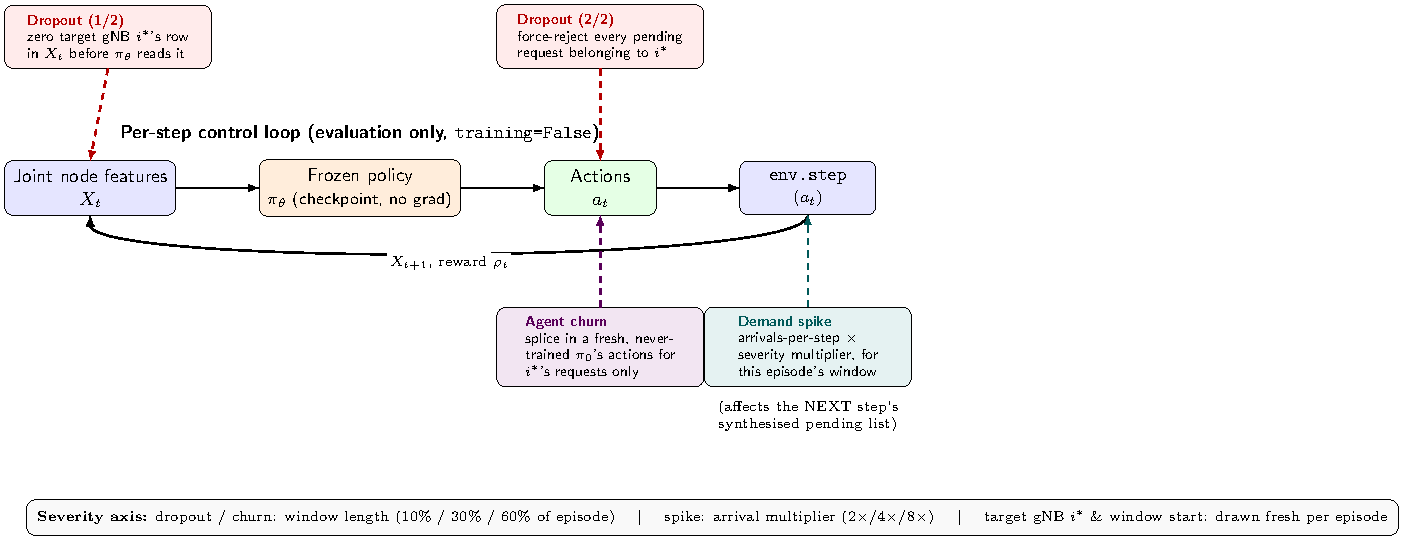
\includegraphics[width=0.92\textwidth]{figures/fig6_m4_disruption_loop.pdf}
\caption{Where each M4 disruption kind intercepts the frozen policy's
per-step evaluation loop. Dropout acts twice (corrupting the target
gNB's input row, then separately forcing that gNB's own requests to
reject, so a policy cannot simply learn around the corrupted feature);
agent churn substitutes a fresh, never-trained policy's actions for the
target gNB only, leaving every other agent's decisions untouched; demand
spike is entirely external to the policy, acting on the arrival process
the environment synthesises for the following step. All three are
evaluation-only perturbations -- the policy itself is never updated.}
\label{fig:m4-injection}
\end{figure*}

\subsection{Dropout and Agent Churn: A Real, Accelerating Threshold Effect}
Fig.~\ref{fig:m4-disruption}(a)-(b) report the normalised-reward cost at
each severity. Dropout costs every arm significantly at every severity
(Wilcoxon $p\leq0.03$, 9 or 10 of 10 seeds hurt in every case), and the
cost accelerates with severity rather than growing proportionally: for
GAT-CTDE, +0.165 at the 10\% window, +0.601 at 30\% (roughly
3.6$\times$ the first increment), +1.710 at 60\% (roughly 1.8$\times$
the second increment) -- the same super-linear pattern holds for every
arm. Agent churn shows the same accelerating shape for GAT-CTDE
(+0.059/+0.200/+0.529, $p=0.0039$ throughout) and the federated arm
(+0.073/+0.240/+0.585, $p=0.0039$ throughout).

Independent DQN's own churn cost needs both samples reported together
to state honestly. On the seeds used throughout the rest of this paper
(900--909), it is small and does not clear conventional significance
(+0.000/+0.168/+0.640, $p=0.084/0.106/0.065$) -- which an earlier pass
of this analysis read as independent DQN being architecturally immune
to churn, reasoning that a policy which never attends to another
agent's features (confirmed by inspection: it reads only its own node's
row) has no coordination benefit a churned peer can take away. An
independent-seed replication (seeds 1000--1009, disjoint from every
other result in this paper) contradicts that reading directly:
independent DQN's churn cost there is significant at every severity
(+0.097/+0.657/+1.223, $p=0.0020$ throughout, 10/10 seeds hurt each
time) and \emph{larger} than GAT-CTDE's or the federated arm's at
matched severities in that sample -- the opposite of immune. The
direction was consistent across both samples throughout (churn always
hurts, never helps); what was wrong was treating a borderline,
underpowered $n=10$ result as a confirmed architectural property. We do
not conclude independent DQN is immune to churn: replacing a trained
agent's own decision-making with an untrained one plausibly degrades
that agent's local performance regardless of whether it ever used
cross-agent coordination, and the combined evidence across both samples
now points that way.

\subsection{Demand Spike: A Different, Cleaner Story}
Fig.~\ref{fig:m4-disruption}(c) shows no threshold at all on block
precision, which stays flat and near-ceiling through the highest tested
multiplier for every arm. The normalised-reward signal (not shown) that
spike \emph{improves} per-request reward is real and reproduces across
both seed samples for GAT-CTDE, independent DQN, and the federated arm
($p\leq0.014$ in both), but we do not read it as better decision-making:
it traces to a specific, understood property of the existing reward
shape (a fixed per-step violation penalty diluted by a larger
denominator once request volume rises, still present after the primary
volume normalisation above, which only corrects the dominant,
much larger effect from the reward's accept-scaling service term) --
block precision, a volume-invariant ratio, is the metric that actually
answers whether spike corrupts decision quality, and it says no.
Single-agent DQN's version of this same reward-based signal is
significant in the original sample ($p=0.0020$ at every severity) but
not in the replication ($p=0.084$) -- direction consistent, significance
sample-dependent, reported as such rather than as an unconditional
finding.

\subsection{Independent-Seed Replication}
Every dropout result above, and GAT-CTDE/the federated arm's churn
costs, were checked against the independent 1000--1009 sample and hold
up in both direction and approximate magnitude -- e.g.\ GAT-CTDE's
dropout costs there are +0.170/+0.552/+1.449, close to the 900--909
sample's +0.165/+0.601/+1.710. The one finding that did not survive
(independent DQN's supposed churn immunity) is reported only in its
corrected form above, not as an initial claim we later walk back --
this section already reflects what replication showed, exactly the
discipline Section~\ref{sec:eval-log-bug} argues for. One caveat the
replication surfaced on the M3 privacy sweep
(Section~\ref{sec:results-m3}) rather than here: block precision's
degradation \emph{exists} in both samples but the exact noise level it
begins at does not (perfect through $\sigma=1.0$ in one 10-seed sample,
already degrading at $\sigma=0.5$ in the other) -- a threshold is real;
its precise location is not a property we would claim generalises
beyond the specific ten seeds it was measured on.

Fig.~\ref{fig:replication-forest} puts every headline paired comparison
in this paper next to its independent-sample counterpart on one axis,
recomputed directly from each sample's own raw evaluation logs rather
than retyped from either sample's summary numbers. Panel (a)'s three
architecture/federation comparisons and panel (b)'s dropout/churn costs
for GAT-CTDE and the federated arm all keep the same sign and a
broadly overlapping confidence interval across samples -- visually, the
committed and fresh estimates sit close together on every row except
one. The exception is independent DQN's churn cost (panel (b), bottom
row, shaded): both samples agree the cost is positive (churn never
helps), but the committed sample's interval reaches down toward zero
while the fresh sample's sits clearly higher and to the right of every
other churn estimate in the panel -- the same reversal
Section~\ref{sec:results-m4}-D reports in numbers, here shown as the one
row that visibly does not track its own sample-to-sample agreement the
other six rows show.

\begin{figure*}[t]
\centering
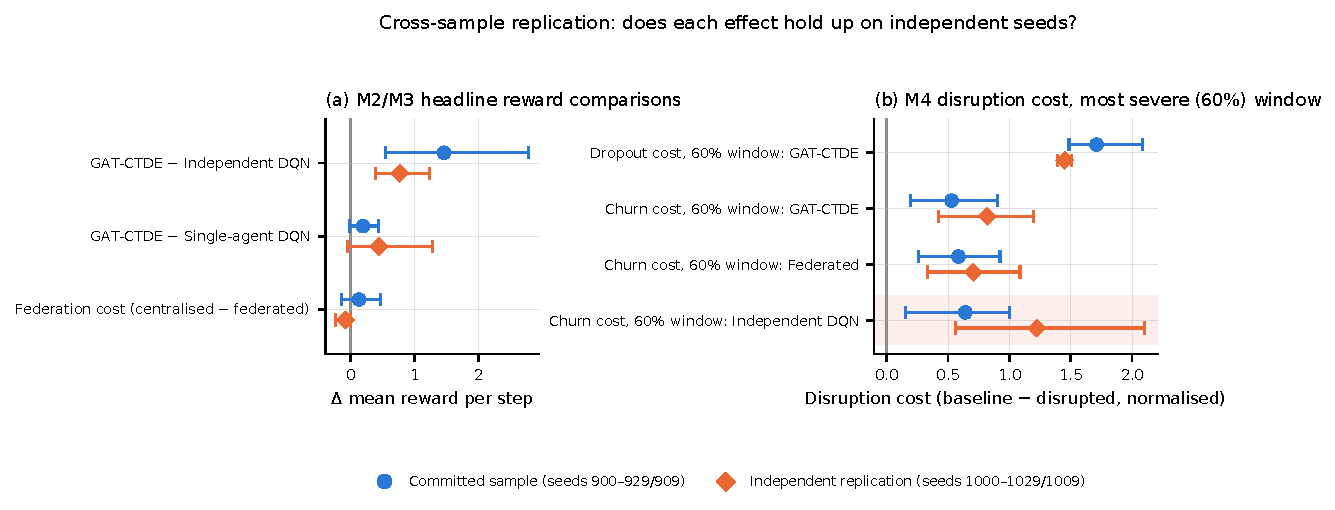
\includegraphics[width=0.92\textwidth]{figures/fig7_replication_forest.pdf}
\caption{Every headline paired comparison in this paper, committed
sample (seeds 900--929/909) against the independent replication sample
(seeds 1000--1029/1009), recomputed from raw logs for both. (a) M2/M3
reward comparisons. (b) M4 disruption cost at the most severe (60\%)
window. The bottom row of (b), independent DQN's churn cost, is the one
comparison whose two samples visibly disagree on more than point-estimate
noise -- the finding retracted in Section~\ref{sec:results-m4}-D.}
\label{fig:replication-forest}
\end{figure*}

\section{Discussion}
Three findings in this paper are, we think, more broadly useful than
the specific architecture: first, that a class-imbalanced, shared
Q-head can silently suppress a minority slice's learning signal in a
multi-slice admission controller, and that per-slice heads are a
simple, verifiable fix; second, that an SLA-compliance metric which
scores decisions only by whether they eventually keep a slice within
its margin -- not by whether the decision itself was correct given the
information available at the time -- can actively reward a degenerate
policy over a correct one whenever the correct action cannot recover
an already-stressed slice's margin. Any admission-control evaluation
in a stress regime where this asymmetry holds should report a
decision-level correctness metric alongside, not instead of, an
outcome-level compliance metric.

Third, that reproducing a result on the same seed and replicating it on
an independent one answer different questions, and only the second
caught a real error in this paper's own analysis. Every number in this
paper was checked for exact, same-seed reproducibility (an eval-log
append bug and an unseeded weight-initialisation path,
Section~\ref{sec:eval-log-bug}, both surfaced and were fixed this way,
neither by inspection alone), which confirms the pipeline is
deterministic but says nothing about whether a finding is real or a
property of one particular sample of seeds. Only the independent-seed
replication in Section~\ref{sec:results-m4} caught the latter: a
claimed architectural immunity to agent churn that read as
``mechanistically sensible'' on one 10-seed sample was directly
contradicted by a second, disjoint one. We would not have caught this
by re-running the same seeds again, however many times, and we think
any paper reporting an architecture-specific claim from a single
seed sample -- ours included, elsewhere, before this check -- should
weigh how much of its evidence is reproduction versus replication.

We are explicit about what remains offline-only. Every result in this
paper uses the 3-gNB offline stress environment; none of it is a live
claim, and Section~\ref{sec:system-model} explains why we do not
believe an offline-trained ranking here would transfer live without
separate verification. Federated learning across three gNBs
under one operator's cluster is also, as configured, a synthetic
privacy scenario -- genuine cross-organisation data separation would
need multiple operators unwilling to pool raw data, which nothing in
our current setup represents. We lead with the operational
coordination benefit of periodic, not per-step, synchronisation
(a real constraint for disaggregated near-real-time RAN Intelligent
Controllers (near-RT RICs) with limited
backhaul, even under one operator) rather than with a privacy
motivation we cannot substantiate at this scale.

\section{Conclusion and Future Work}
\label{sec:conclusion}
We built and iteratively fixed a GAT-CTDE architecture for coordinated
multi-gNB slice admission control, found and diagnosed three failures a
standard compliance metric, an unguarded append-only log, and an
unseeded weight-initialisation path could not have caught on their own
-- a training collapse, a hidden eval-data contamination bug, and a
same-seed-only reproducibility gap -- and showed that on a
correctness-aware reward metric the architecture delivers a decisive,
statistically significant improvement over an independent-learner
ablation, though its edge over our existing single-agent baseline
specifically is small and not decisive at this sample size. Extending
the architecture to federated training with differential privacy, we
found federation to add no measurable reward cost and privacy costly
only past a real threshold in decision precision, not a smooth
trade-off. Evaluating the same frozen policies under mid-episode gNB
dropout, demand spikes, and agent churn, we confirmed the threshold
prediction this paper's own DP-noise finding suggested: dropout and
churn both produce a real, accelerating cost with severity rather than
graceful degradation, while demand spikes do not threshold at all on
the metric that matters, a genuinely different failure mode.
Cross-checking every result against an independent seed sample, not
just the same seeds reproduced again, caught one architectural claim
(that independent DQN is immune to agent churn) that a single sample
had made look confirmed but was not -- retracted before it could
appear as a finding, with the correction reported alongside it rather
than silently.

Everything in this paper is offline-only, and validating whether any of
these architectural or privacy-cost rankings survive contact with a
live testbed -- as our single-agent work already did, and as this
offline environment's own known live-fidelity gap
(Section~\ref{sec:system-model}) says we should not assume -- is the
most direct remaining step. Two narrower questions this paper's own
results raise are also still open: whether the churn-cost gap between
coordination-dependent and independent architectures is itself
statistically real (no formal paired test between architectures'
disruption costs was run here, only each architecture against its own
undisrupted baseline), and why the privacy threshold's exact location
shifted between our two seed samples (Section~\ref{sec:results-m4}) --
whether that reflects genuine sensitivity to which ten seeds are drawn,
or a factor this paper has not identified.

\section*{Acknowledgment}
\authorTODO{Same acknowledgment text as paper\_conf/main.tex, or updated for this paper -- please fill in.}

\bibliographystyle{IEEEtran}
\bibliography{refs}

\end{document}
